\cotefile{97}
\scanpage{2}
% letterhead
\noindent\begin{tabular}[t]{c}
COLLÈGE\\
DE\\
FRANCE\\
\rule{1.8em}{0.5pt}\\
CHAIRE\\
D’ALGÈBRE ET GÉOMÉTRIE
\end{tabular}\hfill
\begin{tabular}[t]{l}
\textit{Paris, le} 4 Nov. 66\\
\end{tabular}

Cher Grothendieck,\\

Je n’ai pas regardé ton pb. Mais je suis tombé sur une ``Notice'' que je t’envoie ci-joint, démontrant la même chose que toi.

La Notice renvoie à un \unsure{papier} de Milnor, que j’ai, où celui-ci regarde justement \unsure{le fibré|les fibrés} à groupe $\mathrm{SL}_{2}$ qui sont plats, et de base une surface. C’est \unsure{très} joli.

Bien à toi\\
J-P. \uline{Serre}.\\
% archive sheet number: 1
\clearpage
\scanpage{3}
\diagram{\begin{tikzcd}[ampersand replacement=\&, /tikz/execute at end picture={
  \begin{scope}[x=.0108cm,y=-.0108cm,line cap=round,line join=round,
      every node/.style={anchor=base west,inner sep=0pt,font=\normalsize}]
    \draw[line width=.4pt] (83,96) ellipse [x radius=.18cm,y radius=.14cm];
    \node at (77,104) {\unsure{1|2}};
    \draw[line width=.85pt] (116,78) -- (50,138);
    \node[font=\small] at (590,134) {\deleted{\unsure{Kleppe|Kleiman}}};
    \draw[line width=.6pt] (595,135) -- (764,130);
    \draw (742,84) ellipse [x radius=.23cm,y radius=.20cm];
    \node[anchor=center] at (742,84) {1};
    \node at (799,135) {\uline{Benjamin}};
    \draw[line width=.8pt] (50,138) .. controls (82,149) and (110,175) .. (143,197);
    \draw[line width=.8pt] (50,138) .. controls (115,208) and (117,268) .. (158,324);
    \draw[line width=.8pt] (50,138) .. controls (61,304) and (57,344) .. (169,372);
    \draw[line width=.8pt] (72,307) .. controls (78,414) and (71,439) .. (173,477);
    \draw[line width=.8pt] (83,414) .. controls (98,528) and (89,536) .. (140,536)
      -- (191,536) -- (191,544);
    \draw (140,164) -- (130,164) .. controls (130,228) and (129,323) .. (140,385) -- (162,379);
    \draw[line width=.9pt] (165,402) -- (144,403) -- (148,556) -- (170,555);
    \draw[line width=.9pt] (183,569) -- (157,571) .. controls (166,663) and (143,794) ..
      (157,920) -- (166,955) -- (199,956);
    \draw (181,575) -- (163,572) -- (161,943) -- (182,941);
    \draw (182,601) -- (159,605) -- (168,935) -- (182,933);
    \draw[line width=.9pt] (208,978) -- (182,979) .. controls (182,1054) and (195,1145) .. (207,1241) -- (229,1238);
    \draw (185,981) -- (190,1084) -- (199,1086);
    \draw (190,1083) -- (198,1164) -- (220,1164);
    \draw (201,1173) -- (201,1236) -- (221,1240);
    \draw (198,656) -- (194,717) .. controls (317,719) and (503,700) .. (633,698);
    \draw (211,646) -- (631,626) -- (626,711);
    \draw (223,858) -- (216,920) .. controls (306,929) and (382,911) .. (435,905);
    \draw (238,855) -- (439,847) -- (429,913);
    \node at (140,124) {Serre};
    \node at (147,195) {Illusie};
    \node at (151,261) {\unsure{Jouanolou}};
    \node at (170,344) {\unsure{Hakim}};
    \node at (178,380) {Giraud};
    \node at (171,427) {Deligne};
    \node at (177,492) {Coates};
    \node at (190,541) {\unsure{Jurmila|Jarmila|Jumila}};
    \node at (224,594) {Artin};
    \node at (196,633) {Tate};
    \node at (211,705) {Rim};
    \node at (356,702) {,};
    \node at (412,686) {Swan};
    \node at (222,765) {Mumford};
    \node at (235,829) {Atiyah};
    \node at (235,912) {Harder};
    \node at (239,951) {Mazur};
    \node at (243,1005) {Milnor};
    \node at (232,1085) {Bass};
    \node at (238,1168) {Tits};
    \node at (263,1224) {Hirzebruch\unsure{,|.}};
  \end{scope}
}] {}
\end{tikzcd}}
% archive sheet number: 2
\clearpage
\scanpage{4}
% letterhead
\noindent\begin{tabular}{c}
INSTITUT\\
DES HAUTES ÉTUDES SCIENTIFIQUES\\
\rule{3.5em}{0.5pt}
\end{tabular}

Dear Atiyah,\\

Can you send \unsure{f|b}
% archive sheet number: 3
\clearpage
\scanpage{8}\mspage{\handwritten{23}}
\makeatletter\tagsleft@true\makeatother
\[
  0 \handwritten{\longrightarrow} \underline{\mathrm Z}/\handwritten{\delta''}\,\underline{\mathrm Z}
  \handwritten{\longrightarrow \mathord{\tikz[x=1em,y=1ex,baseline=0pt,line width=.045em,line cap=round]{\draw (0,.08)--(.88,.08) (0,1.43)--(.88,1.43) (.19,.08)--(.19,1.43) (.44,.08)--(.44,1.43) (.69,.08)--(.69,1.43);}}'}(Y,\underline A)
  \handwritten{\longrightarrow \mathord{\tikz[x=1em,y=1ex,baseline=0pt,line width=.045em,line cap=round]{\draw (0,.08)--(.88,.08) (0,1.43)--(.88,1.43) (.19,.08)--(.19,1.43) (.44,.08)--(.44,1.43) (.69,.08)--(.69,1.43);}}^{\deleted{\unsure{\prime|*}}}}(Y,\underline B)
  \handwritten{\longrightarrow} 0 \quad . \tag*{(4.38)}
\]

Explicitons deux cas particuliers importants:

\deleted{(\unsure{4.6})}
\uline{Cas particulier} \deleted{\unsure{:|1}}\inserted{(4.6):} $Y$ \uline{est une courbe algébrique sur un corps algébriquement clos}. Alors la \deleted{relation (4.13) est automatiqu\unsure{e.|e. La}} plus grande partie de la discussion précédente devient triviale. La relation (4.13) est automatiquement satisfaite, et on a (4.12 bis) :
\[
  \unsure{\mathbb{B}\mathrm r|\mathrm{Br}}(X)\handwritten{\overset{\sim}{\longrightarrow}}H^{1}(Y,\underline B)\quad ; \tag*{(4.39)}
\]
lorsque de plus les $\handwritten{\delta}_{y}$ sont égaux à $1$, i.e. \handwritten{si} $X$ n'a pas de fibre multiple sur $Y$, alors le deuxième membre s'explicite \deleted{comme étant égal à} par
\[
  0\handwritten{\longrightarrow}\underline{\mathrm Z}/\handwritten{\delta}\underline{\mathrm Z}
  \handwritten{\longrightarrow}H^{1}(Y,\underline{\deleted{\unsure{X|B}}\handwritten{A}})
  \handwritten{\longrightarrow}H^{1}(Y,\underline B)\handwritten{\longrightarrow}0\quad , \tag*{(4.40)}
\]
compte tenu que \deleted{dans} l'on a ici nécessairement $\handwritten{\delta}=\handwritten{\delta'}=\handwritten{\delta''}$ .

\uline{Cas particulier} (4.7): $Y$ \uline{est une courbe algébrique propre sur un corps fini} $k$. Ici encore, (4.13) \deleted{\unsure{et (4.16)}}\deleted{\unsure{sont}}\handwritten{est} automatiquement satisfaite, $k$ étant parfait, \deleted{\unsure{et}}\inserted{\handwritten{ainsi que (4.16) puisque $k(y)$ est de dimension $\leq 1$, d'où $H^{3}(k(y),G_{\mathrm m})=0$; de plus}} on aura $\handwritten{\delta}=\handwritten{\delta'}\handwritten{\deleted{\unsure{=\delta''}}}$, et de même pour les invariants hensélisés et strictement hensélisés. Comme on a encore $\mathrm{Br}(Y)=0$, on trouve ici (4.4):
\[
  0\handwritten{\longrightarrow}\mathrm{Br}(X)\handwritten{\longrightarrow \mathord{\tikz[x=1em,y=1ex,baseline=0pt,line width=.045em,line cap=round]{\draw (0,.08)--(.88,.08) (0,1.43)--(.88,1.43) (.19,.08)--(.19,1.43) (.44,.08)--(.44,1.43) (.69,.08)--(.69,1.43);}}}(Y,\underline B)
  \handwritten{\longrightarrow}\underline{\deleted{\unsure{2|Z}}\handwritten{\mathrm Z}}/\deleted{\unsure{1|\delta}}\handwritten{\Delta}\underline{\mathrm Z}
  \handwritten{\longrightarrow}0\quad ,\qquad\text{où}\quad\handwritten{\Delta\mid\delta}\quad . \tag*{(4.41)}
\]
\deleted{\unsure{compte tenu de|compte tenu du}} D'autre part, si les $\handwritten{\delta}_{y}$ sont égaux à $1$, i.e. si le morphisme déduit de $f:X\handwritten{\longrightarrow}Y$ en passant à la clôture algébrique de $k$ n'a pas de fibre multiple, alors on trouve la suite exacte
\[
  0\handwritten{\longrightarrow}\underline{\mathrm Z}/\handwritten{\delta''}\underline{\mathrm Z}
  \handwritten{\longrightarrow \mathord{\tikz[x=1em,y=1ex,baseline=0pt,line width=.045em,line cap=round]{\draw (0,.08)--(.88,.08) (0,1.43)--(.88,1.43) (.19,.08)--(.19,1.43) (.44,.08)--(.44,1.43) (.69,.08)--(.69,1.43);}}}(Y,\underline A)
  \handwritten{\to \mathord{\tikz[x=1em,y=1ex,baseline=0pt,line width=.045em,line cap=round]{\draw (0,.08)--(.88,.08) (0,1.43)--(.88,1.43) (.19,.08)--(.19,1.43) (.44,.08)--(.44,1.43) (.69,.08)--(.69,1.43);}}}(Y,\underline B)\handwritten{\longrightarrow}0\quad , \tag*{(4.42)}
\]
ce qui est un cas particulier de (4.37), compte tenu de\deleted{s} \inserted{\handwritten{la}} relation\deleted{s} suivante\deleted{s}\unsure{:}
\[
  \handwritten{\bar{\delta}}_{y}=\handwritten{\delta}_{y} \tag*{(4.43)}
\]
pour tout point fermé $y$ de $Y$, qui implique ici $\handwritten{\bar{\delta}}_{y}=1$ d'où $\handwritten{\mathord{\tikz[x=1em,y=1ex,baseline=0pt,line width=.045em,line cap=round]{\draw (0,.08)--(.88,.08) (0,1.43)--(.88,1.43) (.19,.08)--(.19,1.43) (.44,.08)--(.44,1.43) (.69,.08)--(.69,1.43);}}'}(Y,\underline A)=\handwritten{\mathord{\tikz[x=1em,y=1ex,baseline=0pt,line width=.045em,line cap=round]{\draw (0,.08)--(.88,.08) (0,1.43)--(.88,1.43) (.19,.08)--(.19,1.43) (.44,.08)--(.44,1.43) (.69,.08)--(.69,1.43);}}}(Y,\underline A)$.

La démonstration de\deleted{s} \handwritten{l'}égalité\deleted{s} (4.43), qui est une conséquence facile du
\reversemarginpar\margin{\handwritten{\unsure{x|$\times$}}}\normalmarginpar
théorème de \deleted{Lang}\handwritten{LANG} \inserted{\handwritten{[24] $H^{1}(k,G)=0$}} pour le corps fini $k(y)$ et le schéma de Picard \deleted{\unsure{con}}\handwritten{con}nexe $\handwritten{G=}\underline{\mathrm{Pic}}^{0}_{X_{y}/y}$, est laissé\handwritten{e} au lecteur comme un exercice plaisant et délectable.
% archive sheet number: 7
\clearpage
\scanpage{10}\mspage{\handwritten{17}}
$H^{3}(Y,\underline G_{\mathrm m})\handwritten{\simeq}\underline{\mathrm Q}/\underline{\mathrm Z}$, d'où le corollaire.

Soit \deleted{\unsure{$i$:}}
\[
  i:\handwritten{\unsure{\eta|y}\longrightarrow}Y
\]
l'inclusion du point générique, et posons
\[
  \underline B=i_{\handwritten{\unsure{\times|\ast}}}(i^{*}(P)) \quad , \tag*{(4.8)}
\]
de sorte qu'on a un homomorphisme canonique
\[
  P\handwritten{\longrightarrow}\underline B \quad , \tag*{(4.9)}
\]
et on posera
\[
  \underline E=\operatorname{Ker}(P\handwritten{\to}\underline B)
  \quad ,\quad \underline F=\operatorname{Coker}(P\handwritten{\to}\underline B)\quad . \tag*{(4.10)}
\]

Les faisceaux $\underline E$ et $\underline F$ sont des ``faisceaux gratte-ciel'' , qui sont donc connus lorsqu'on connait leurs restrictions aux points fermés de $Y$. Leur\handwritten{s} fibre\handwritten{s} géométriques au dessus d'un tel point $y$ s'obtiennent comme les noyaux et conoyau de l'homomorphisme
\[
  \deleted{\unsure{\mathrm{Pic}(}}\inserted{\mathrm{Pic}(\overset{\handwritten{\sim}}{X})=}
  \mathrm{Pic}(\overset{\handwritten{\sim}}{X}/\overset{\handwritten{\sim}}{Y})\handwritten{\longrightarrow}
  \mathrm{Pic}(\overset{\handwritten{\sim}}{X}_{\handwritten{\tilde\eta}}/\handwritten{\tilde\eta})\quad ,
\]
où les $\handwritten{\sim}$ dénotent l'effet de la localisation stricte relativement à un point géométrique $\bar y$ au dessus de $y$. \deleted{\unsure{Lorsque}} Compte tenu que \deleted{L}\handwritten{l}e morphisme précédent se factorise par le sous-groupe $\mathrm{Pic}(\overset{\handwritten{\sim}}{X}_{\handwritten{\eta}})$, et que $\mathrm{Pic}(\overset{\handwritten{\sim}}{X})\handwritten{\longrightarrow}\mathrm{Pic}(\overset{\handwritten{\sim}}{X}_{\handwritten{\tilde\eta}})$ est surjectif puisque $\overset{\handwritten{\sim}}{X}$ est régulier, on trouve
\[
  \deleted{\underline{\unsure{E|F}}_{\bar y}}\qquad
  \underline F_{\bar{\deleted{\unsure{y}}\handwritten{y}}\deleted{\unsure{*}}}=
  \mathrm{Pic}(\overset{\handwritten{\sim}}{X}_{\handwritten{\eta}}/\handwritten{\tilde\eta})\,/\,\mathrm{Pic}(\overset{\handwritten{\sim}}{X}_{\handwritten{\tilde\eta}}) \tag*{(4.11)}
\]
\[
  \underline E_{\bar y}\deleted{\unsure{\delta_y|y}}=
  \operatorname{Ker}\bigl(\mathrm{Pic}(\overset{\handwritten{\sim}}{X})\handwritten{\longrightarrow}\mathrm{Pic}(\overset{\handwritten{\sim}}{X}_{\handwritten{\tilde\eta}})\bigr)\quad . \tag*{(4.12)}
\]
Compte tenu que $\mathrm{Br}(\handwritten{\tilde\eta})=0$ si $k(y)$ est parfait, et que c'est un groupe de $p(y)$-torsion en tous cas, où $p(y)$ est l'exposant cara\deleted{\unsure{tc}}\handwritten{ct}éristique de $k(y)$, on trouve que $\underline F_{\bar y}$ est un groupe de $p(y)$-torsion, nul si $k(y)$ est parfait, Désignant par $\handwritten{\delta}_{y},\handwritten{\delta'}_{y},\handwritten{\delta''}_{y}$ les entiers analogues à $\handwritten{\delta},\handwritten{\delta'},\handwritten{\delta''}$ pour la situation localisée $\overset{\handwritten{\sim}}{X}\handwritten{\longrightarrow}\overset{\handwritten{\sim}}{Y}$, un argument déjà \deleted{\unsure{sig}} fait plus haut nous montre que $\underline F_{\bar y}$ \deleted{est nul \unsure{également}} est nul également si $\handwritten{\delta}_{y}=1$, par exemple si $\overset{\handwritten{\sim}}{X}$ admet un\unsure{e} section sur $\overset{\handwritten{\sim}}{Y}$. Nous allons supposer pour simplifier, par la suite, que
% archive sheet number: 9
\clearpage
\scanpage{14}\mspage{\handwritten{20}}
\[
  \handwritten{\mu}^{i}_{y},\quad{\handwritten{\unsure{\nu|v}}}^{i}_{y}
  \tag*{(4.1\deleted{7}\handwritten{9})}
\]
la multiplicité radicielle et la multipli\makebox[0pt][l]{\raisebox{-.72em}[0pt][0pt]{\scriptsize\unsure{;|,}}}cité séparable de $C^{i}_{\deleted{i}y}$ sur $k(y)$ respectivement
\reversemarginpar\margin{\handwritten{\unsure{x|$\times$}}}\normalmarginpar
(EGA IV 4\handwritten{.7.4.} ), - donc $\handwritten{\mu}^{i}_{y}=1$ si $k(y)$ est par\deleted{\unsure{a}}fait.

On \deleted{pose aussi} considère aussi la plus petite extension galoisienne $k(y)^{i}$
\[
  \deleted{Z^{i}_{y}=\operatorname{Spec}(H^{0}(X^{i}_{y\,\mathrm{réd}},\underline O_{X^{i}_{y\,\mathrm{réd}}}))}
  \deleted{\,,\qquad Z=\unsure{\textstyle\prod}_{i}Z^{i}_{y}\,,}
  \tag*{\deleted{(4.18)}}
\]
\deleted{de sorte que l'on a simplement $Z^{i}_{y}$ est le spectre d'une extension finie $k(y)_{i}$ de $k(y)$, de degré séparable} de $k(y)$ tel que les composantes irréductibles de $(X^{i}_{y})\otimes_{k(y)} k(y)^{i}$ soient géométriquement irréductibles: c'est une extension finie\inserted{\handwritten{ de $k(y)$,}} de degré $\handwritten{\nu}^{i}_{y}$. On pose
\reversemarginpar\margin{\handwritten{\unsure{---|$\sim$}}}\normalmarginpar
\[
  Z^{i}_{y}=\operatorname{Spec}(k(y)^{i}),\qquad
  Z_{\deleted{\unsure{x|i}}y}=\handwritten{\textstyle\prod}Z^{i}_{y}\quad\deleted{\unsure{,}}\handwritten{\unsure{;|.}}
  \tag*{(4.\deleted{18}\handwritten{20})}
\]
Ceci posé, le faisceau $\underline E_{y}$ sur $y$ s'insère dans une suite exacte de faisceaux
\[
  0\handwritten{\to}\underline{\mathrm Z}_{y}\handwritten{\longrightarrow}
  p_{y\handwritten{*}}(\underline{\mathrm Z}_{Z_{y}})\handwritten{\to}
  \underline E_{y}\handwritten{\longrightarrow}0\quad ,
  \tag*{(4.\deleted{19}\handwritten{21})}
\]
où $p_{y}:Z_{y}\handwritten{\longrightarrow}y$ est la projection structurale, et où l'homomorphisme $\underline{\mathrm Z}_{y}\handwritten{\longrightarrow}p_{y\handwritten{*}}(\underline{\mathrm Z}_{Z_{y}})$ est adjoint de l'homomorphisme
\[
  p_{y}^{\handwritten{*}}(\underline{\mathrm Z}_{y})=\underline{\mathrm Z}_{Z}
  \handwritten{\longrightarrow}\underline{\mathrm Z}_{Z_{\deleted{\unsure{y}}}}
  \tag*{(4.2\deleted{0}\handwritten{2})}
\]
qui, sur la composante $Z^{i}_{y}$, se réduit à la multiplication par $a^{i}_{y}$. La suite exacte de cohomologie associée à (4.\deleted{19}\handwritten{21}) nous fournit alors
\[
\begin{aligned}[t]
  H^{1}(y,\underline E_{y})&=\deleted{\unsure{\mathrm{Co}}}\operatorname{Ker}
  \bigl(H^{2}(y,\underline{\mathrm Z}_{y})\handwritten{\longrightarrow\textstyle\prod_{i}}
  H^{2}(Z^{i}_{y},\underline{\mathrm Z})\bigr)\\
  &=\deleted{\unsure{\mathrm{Co}}}\operatorname{Ker}
  \bigl(H^{1}(y,\underline{\mathrm Q}/\underline{\mathrm Z})\handwritten{\to}
  \handwritten{\deleted{\unsure{\to}}\textstyle\prod_{i}}H^{1}(Z^{i}_{y},\underline{\mathrm Q}/\underline{\mathrm Z})\bigr)\quad ,
\end{aligned}
\tag*{(4.2\deleted{1}\handwritten{3})}
\]
où la flèche $H^{1}(y,\underline{\mathrm Q}/\underline{\mathrm Z})\handwritten{\longrightarrow}H^{1}(Z^{i}_{y},\underline{\mathrm Q}/\underline{\mathrm Z})$ est l'homomorphisme de tra\deleted{\unsure{o}}\handwritten{n}\deleted{\unsure{i}}sition évident, multiplié par $a^{i}_{y}$. Comme $H^{1}(y,\underline E_{y})$ est l'intersection des noyaux de ces homomorphismes, \deleted{\unsure{dont chacun}}\inserted{et qu'un tel noyau} est manifestement annulé par $a^{i}_{y}\handwritten{\nu}^{i}_{y}$\deleted{\unsure{e}}, on voit que $H^{1}(y,\underline E_{y})$ est annulé par
\[
  d_{y}=\operatorname{pgcd}(a^{i}_{y}\handwritten{\nu}^{i}_{y})\deleted{\unsure{;}}.
  \tag*{(4.2\deleted{2}\handwritten{4})}
\]

Lorsque $k(y)$ est fini, ou plus généralement pseudo-fini au sens de Serre, i.e. son groupe fondamental $\operatorname{Gal}(\overline{k(y)}/k(y))$ isomorphe à $\overset{\handwritten{\scriptscriptstyle\wedge}}{\underline{\mathrm Z}}$, alors on t\deleted{\unsure{o}}rouve
% archive sheet number: 13
\clearpage
\scanpage{19}\mspage{- IV- \handwritten{1102} -}
(21.6.5) Considérons donc un diviseur \uline{positif} $D^{\unsure{\prime}}$ sur $X$\inserted{ ($X$ é\deleted{\unsure{n}}tant supposé \uline{noethérien})}, de sorte que l'Idéal \inserted{fractionnaire} $\underline I_{X}(D)$ est un \uline{Idéal de} $\underline O_{X}$, qui est un $\underline O_{X}$-Module \uline{inversible}; soit $Y(D)$ le sous-préschéma fermé de $X$ qu'il définit. \deleted{\unsure{Cela signifie}}\inserted{Pour} \deleted{\unsure{qu}} tout $x\handwritten{\in}Y(D)$, \deleted{\unsure{que,}} il y a par hypothèse un voisinage \inserted{\handwritten{ouvert}} $U$ de $x$ dans $X$ et une section \uline{régulière} $t\handwritten{\in\Gamma}(U,\underline O_{X})$ telle que $\underline I_{X}(D)\handwritten{\mid}U=\underline O_{U}\mathbin{.}t$ (21.2.7) ; en d'autres termes, l'immersion canonique $Y(D)\handwritten{\to}X$ est \uline{régulière et de codimension 1} \inserted{(19.1.4) en tout point de $Y( D)$}. On notera d'ailleurs qu'inversement, si $Y$ \reversemarginpar
% slanted
\margin{\figure{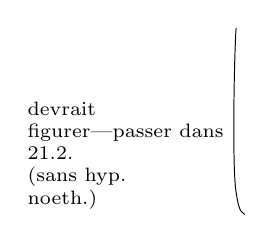
\begin{tikzpicture}[x=1em,y=1em,baseline=0pt]
  \node[anchor=north east,align=left,inner sep=0pt,font=\scriptsize] at (0,0)
    {\handwritten{\unsure{devrait}}\\
     \handwritten{\unsure{figurer|passer} dans}\\
     \handwritten{21.2.}\\
     \handwritten{(\unsure{sans} \unsure{hyp.}}\\
     \handwritten{\unsure{noeth.})}};
  \draw[line width=.35pt] (.43,2.65) .. controls (.36,1.6) and (.29,-2.25) .. (.42,-3.2)
     .. controls (.49,-3.7) and (.55,-4) .. (.74,-4.08);
\end{tikzpicture}}}
est un sous-préschéma fermé de $X$, régulièrement immergé dans $X$ et \deleted{\unsure{est}} de codimension $1$ en tout point de $Y$, il existe un diviseur positif et un seul \deleted{\unsure{préschéma|positif}} $D$ sur $X$ tel que $Y(D)=Y$, car\deleted{\unsure{ cela signifie}}\inserted{ pour} \deleted{\unsure{qu}} tout $x\handwritten{\in}Y$, il y a un voisinage $U$ de $x$ dans $X$ tel que $Y\handwritten{\cap}U$ soit défini par un Idéal de $\underline{\unsure{\mathbb O|O}}_{U}$ de la forme $\underline O_{U}\mathbin{.}t$, où $t$ est \uline{réguli\deleted{\unsure{re}}\handwritten{er}} dans $\handwritten{\Gamma}(U,\underline O_{X})$.


Puisque $X$ est supposé noethérien, $Y(D)$ n'a qu'un nombre fini de points maximaux, et en chacun de ces points $x$, on a $\operatorname{codim}(\handwritten{\{}x\handwritten{\}},X)={}\allowbreak{}=\operatorname{dim}(\underline O_{X,x})=1$, autrement dit $x\handwritten{\in}X^{(1)}$ ;
% slanted
\margin{\handwritten{\uline{réf} !}}\normalmarginpar
\deleted{\illegible{2} \unsure{partie} \illegible{1}} en outre, $\underline O_{Y(D),x}$ est un anneau \uline{artinien} en chacun de ces poi\deleted{\unsure{g}}nts. En tout point $x\handwritten{\in}X^{(1)}$ qui n'est pas point maximal de $Y(D)$, on a nécessairement $x\handwritten{\notin}Y(D)$, donc $\underline O_{Y(D),x}=0$. Posons
\[
  \operatorname{cyc}(D)=\handwritten{\sum}^{\handwritten{\unsure{\prime}}}_{x\handwritten{\in}X^{(1)}}
  \operatorname{long}(\underline O_{Y(D),x})\mathbin{.}\handwritten{\overline}{\handwritten{\{}x\handwritten{\}}}
  \tag*{(21.6.5.1)}
\]
qui est donc un élément de $Z^{1}\llap{\raisebox{-.12ex}[0pt][0pt]{\tiny\unsure{.}}}(X)$.

\uline{Proposition} (21.6.6) .- \deleted{\uline{Si} $X$ \uline{est noethérien},} \uline{\deleted{l}\handwritten{L}'application} $D\handwritten{\leadsto}\operatorname{cyc}(D)$\deleted{\unsure{;}} \uline{est un homomorphisme du monoïde} $\operatorname{Div}^{+}(X)$ \uline{dans} $Z^{1}(X)$ .

Tout revient à voir que pour deux diviseurs \uline{positifs} $D,D'$, on a $\operatorname{cyc}(D+D')=\operatorname{cyc}(D)+\operatorname{cyc}(D')$. Or, on a (21.2.5) $\underline I_{X}(D+D')=\underline I_{X}(D)\underline I_{X}(D')$; tout revient à voir que si $x\handwritten{\in}X^{(1)}$, \inserted{\handwritten{si l'on pose}} $A=\underline O_{X,x}$, et si $t$ et $t'$ sont deux éléments réguliers de $A$, on a $\operatorname{long}(A/tt'A)=\operatorname{long}(A/tA)+{}\allowbreak{}+\operatorname{long}(A/t'A)$ ; mais puisque \deleted{\unsure{$x$}} $t$ est régulier, $tA/tt'A$ est isomorphe à $A/t'A$, d'où \deleted{\unsure{résulte}} aussitôt la proposition.

Il résulte aussitôt des définitions que pour tout ouvert $U\handwritten{\subset}X$, on
% archive sheet number: 18
